\chapter{Induzione}
L'induzione è una vera e propria rivolzione del modo di ragionare nella logica matematica.
Questo perchè permette di trattare su successioni infinite, o quantomeno illimitate, con un metodo finitario.
Facciamo un'esempio per capire meglio:
\begin{example}\label{ex:induzione}
    Dimostrare che la somma di tutti i naturali da 0 ad n, è data dalla formula:\begin{equation}\label{eq:induzione}
        \sum_{i=0}^ni=\frac{n(n+1)}{2}
    \end{equation}
    Possiamo ovviamente provare con qualche caso utilizzando la formula data:
    \begin{center}
    \begin{tabular}{c|c}
         $n$ & $\sum$ \\\hline
         $0$ & $0$ \\
         $1$ & $1$ \\
         $2$ & $3$ \\
         $3$ & $6$ \\
         $4$ & $10$
    \end{tabular}
    \end{center}
    ma non possiamo procedere in questo modo  all'inifinito. Serve infatti un metodo che ci permette di dimostrare la condizione \ref{eq:induzione}.
\end{example}
Ciò è possibile tramite il processo di induzione, il quale afferma che se una proprietà vale per il primo numero e, valendo per un certo numero, allora vale anche per il successivo, allora vale per tutti i numeri.

Cerchiamo ora di formalizzare questo concetto. Indichiamo dunque con il simbolo $P (n)$ la proposizione da provare per tutti i numeri naturali e presentiamo la dimostrazione per induzione di $P (n)$ in due fasi distinte:
\begin{enumerate}
    \item \textbf{Caso base:} verifica che la condizione valga per il minimo degli indici (generalmente $P(0)$);
    \item \textbf{Passo induttivo:} si ammette la verità di $P (n)$ e, sulla base di ciò, si dimostra che la proposizione $P$ è vera anche per l’indice $n + 1$.
\end{enumerate}

In questo modo se dimostro che la proprità è verificata per tutti i numeri. La prima fase, infatti, ci consente di affermare che la proposizione $P (n)$ è vera per $n=0$; sulla base di ciò, la seconda fase ci assicura che $P (n)$ è vera anche per $n= 1$ (ovvero per il successivo di 0). Appurato ciò, possiamo affermare che $P(n)$ è vera anche per $n = 2$ e così di seguito per tutti gli indici naturali.

\section*{Dimostrazioni per induzione}
\begin{example}
    Riprendiamo l'Esempio \ref{ex:induzione}, dove vogliamo dimostrare che la somma $S(n)$ di tutti i numeri naturali fino ad n è data dalla formula:
    \begin{center}
        $S_n=\frac{n(n+1)}{2}$
    \end{center}
    Procediamo per induzione sull’indice n.
    \begin{enumerate}
        \item Caso base: mostriamo che la formula è verificata per il naturale $n = 0$. $0=\frac{0*1}{2}$
        \item Passo induttivo: ammettiamo ora che la formula in questione sia verificata per l’indice n; ammettiamo cioè che sia vero che
        \begin{center}
            $S_n=\frac{n(n+1)}{2}$
        \end{center}
    \end{enumerate}
    Dovremo, sulla base di ciò, provare la validità della formula anche per l’indice $n +1$. Visto che $S_{n+1} = Sn + (n +1)$, abbiamo che:
    \begin{center}
        $S_{n+1}=\frac{n(n+1)}{2}+n+1=\frac{n(n+1)+2(n+1)}{2}=\frac{(n+1)(n+2)}{2}$
    \end{center}
    Così facendo abbiamo dimostrato che la validità della formula per l’indice $n$ comporta la validità della formula per l’indice $n + 1$. Ciò, unito alla provata validità della formula per $n = 0$, completa la dimostrazione per induzione.
\end{example}
\section{Induzione completa}
Un’apparente generalizzazione del principio di induzione è il principio di induzione completa. 
Se l'ipotesi vale $P (0)$ e, se per ogni $n < m$, la validità di $P (n)$ implica la validità di $P (m)$, allora vale $P (k)$ per ogni $k$.
In questo modo supponiamo che la proprietà valga per tutti i precedenti. Ma analizziamo meglio quanto scritto con un esempio.
\begin{example}
    Vogliamo dimostrare per induzione che il numero di nodi in un qualsisi albero ricorsivo è pari al numero degli archi +1.
    
    \begin{center}
    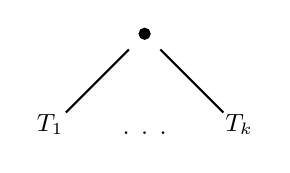
\begin{tikzpicture}
        \draw[thick] (0.2,-0.2) -- (1,-1);\draw[thick] (-0.2,-0.2) -- (-1,-1);
        \filldraw[black] (0,0) circle (2pt);
        \draw (-1.2,-1.4) -- (-1.2,-1.4) node [above] {\small{$T_1$}};\draw (1.2,-1.4) -- (1.2,-1.4) node [above] {\small{$T_k$}};
        \draw (0,-1.4) -- (0,-1.4) node [above] {\small{. . .}};
    \end{tikzpicture}
    \end{center}
    
    Come sempre dimostriamo il caso base, ottenendo 1 nodo e 0 archi.
    Successivamente dimostriamo per passo induttivo. Disegnando un qualsiasi albero ed eliminando una radice, otteniamo due sotto-alberi. Possiamo dimostrare la nostra tesi per i due alberi più piccoli per infine dimostrare che la tesi vale per l'unione dei due o più alberi figli.
\end{example}
